% !TEX root = ../thesis-example.tex
%
%************************************************
% Kern der Arbeit
%************************************************
\chapter{Reranking mittels Click-Trough-Rate Ergebnis}
\label{sec:Reranking}

%Prozessaufbau des Lösungsansatzes
%----------------------------------------------------------------

\section{Prozessaufbau des Lösungsansatzes}
\label{sec:Reranking:Prozessaufbau}

\subsection{Prozessaufbau als Bild}
\label{sec:Reranking:Prozessaufbau:ProzessaufbauBild}

\begin{figure}[H]
\centering
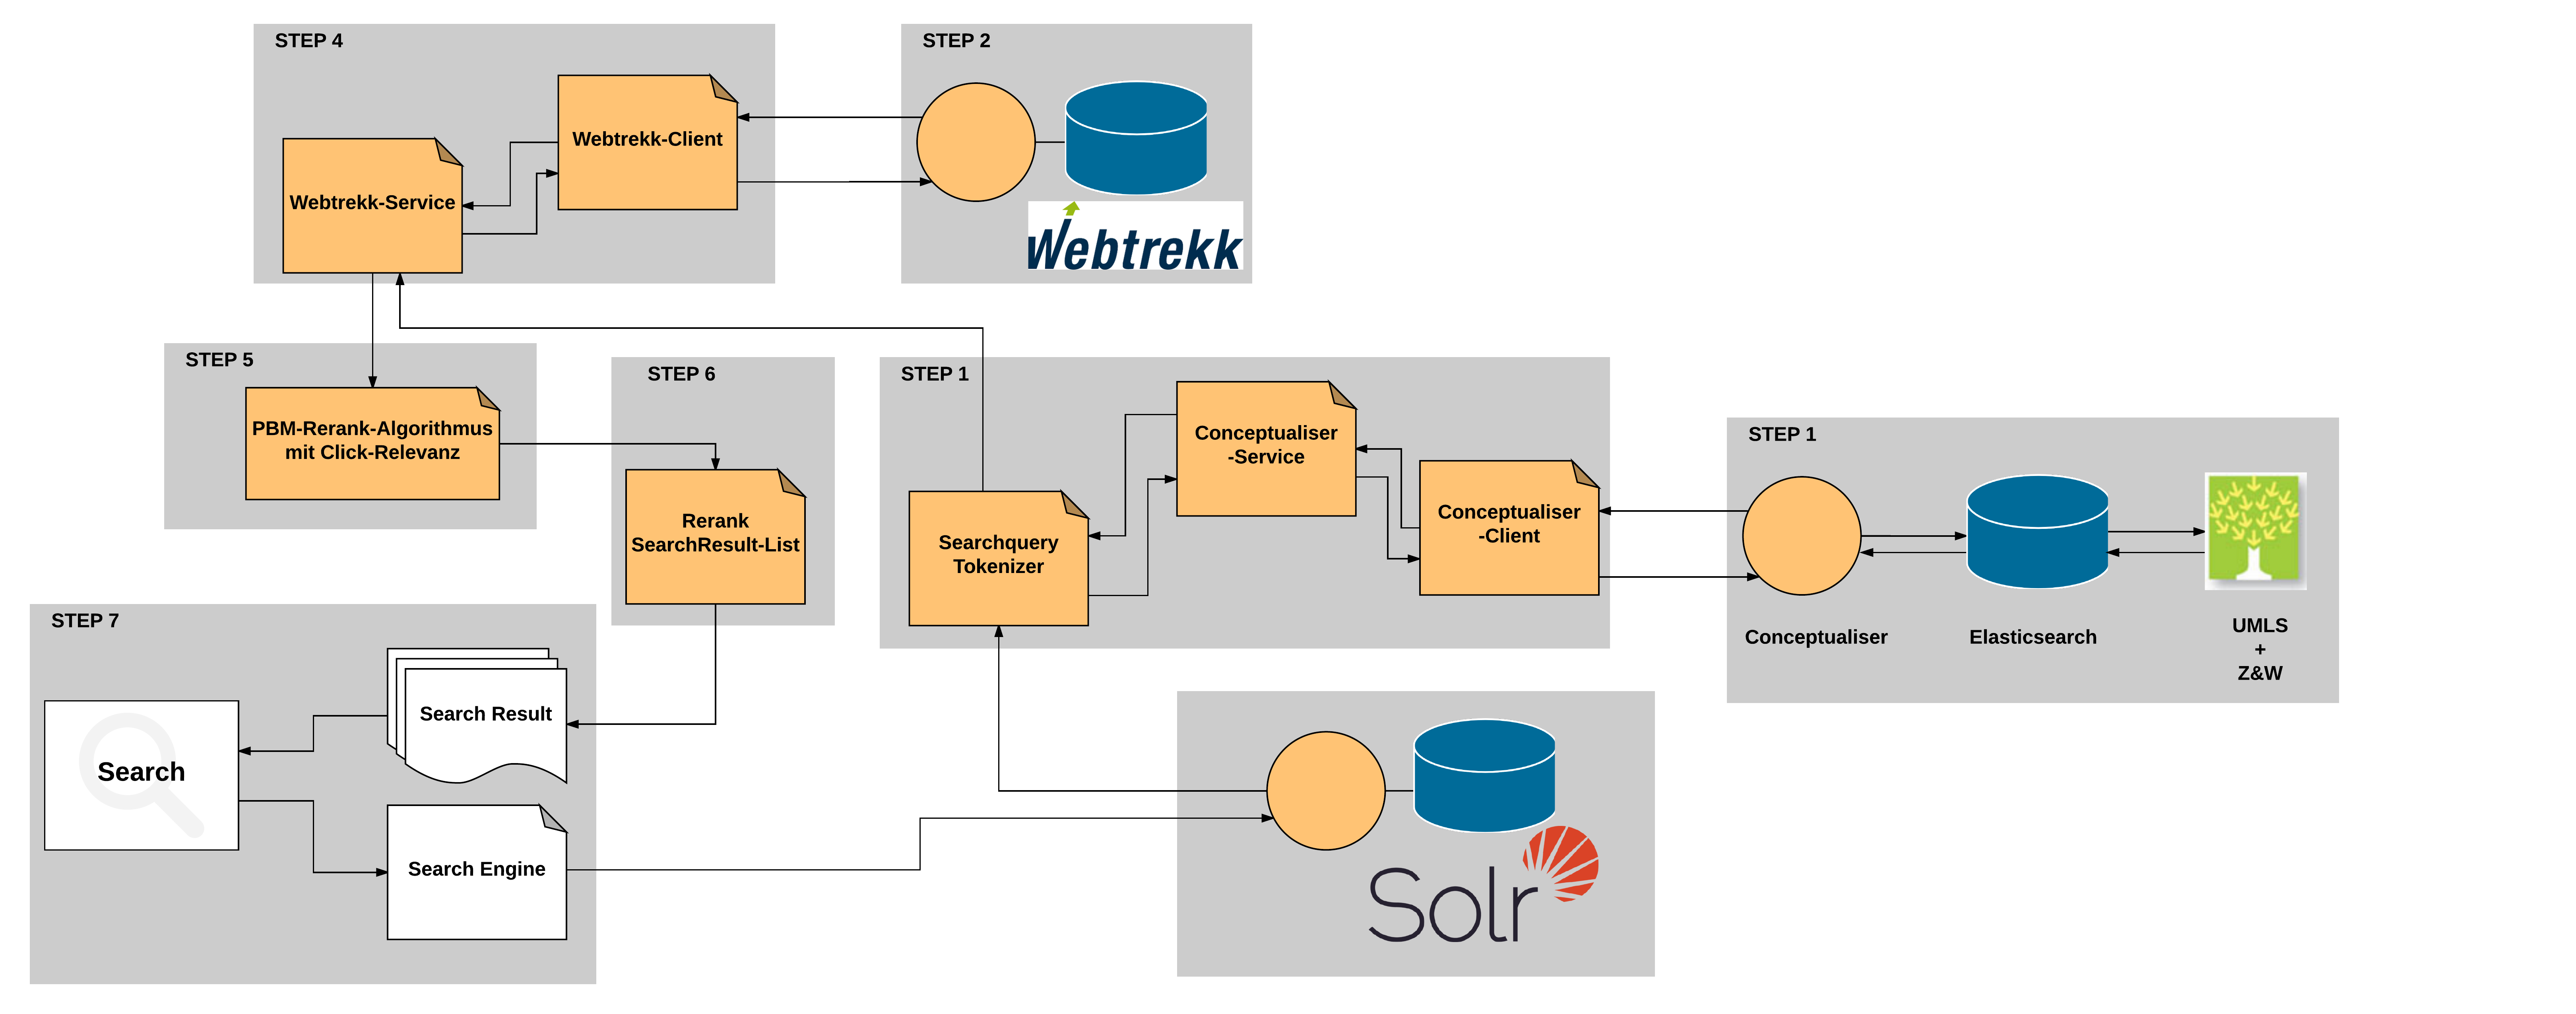
\includegraphics[width=0.5\linewidth]{gfx/Prozessaufbau}
\caption[Prozessaufbau des Lösungsansatzes]{Prozessaufbau des Lösungsansatzes}
\label{fig:SucheSpringerNature}
\end{figure}

\subsection{Daraus entstehende Probleme}
\label{sec:Reranking:Prozessaufbau}

\subsection{Suchterm Segmentierung}
\label{sec:Reranking:Prozessaufbau:SuchtermSegmentierung}

- Was wird gesucht und zu welchem Zweck
	Beispielsweise Zeitschrift => direkter Link auf Zeitschrift
	Oder Kurs (sehr tagesaktuell)
	=> nicht Kern der Arbeit
- Mehrdeutigkeiten
- verwandte Begriffe und Synonyme
- Segmentierung

- Contentprobleme:
--------------------------
- Mehrfachverwertung des Contents => Mehrfache Ausspielung der gleichen Artikel
		Grundsätzlich tritt dieses Problem bei allen Suchanfragen auf - z.B. auch bei den Anfragen COPD, Osteoporose, Sarkoidose und Schilddrüsenkarzinom.
		Für dieses Problem gibt es eine einfache Erklärung: News und kommentierte Studien laufen oft erst online und werden dann z.B. von der MMW, der PneumoNews und 
		der InfoDiab zweitverwertet. Auf diese Weise taucht ein Text dann halt 2-4-6 mal  auf …
		"Außerdem hätte ich gleich noch eine Frage. Bei den Suchanfragen wird mir zum Teil ein und derselbe Artikel gleich mehrfach präsentiert – was auch an der hier im 
		Hause praktizierten Mehrfachverwertung liegt. Auf diese Weise sind dann vier von zehn Suchergebnissen identisch. Willst du das wirklich so haben?"

- Ausspielung von Teaser => Contentproblem
	Vielleicht noch eine Anmerkung zu „Teaser“ Ich denke, dass der Begriff jeden ernsthaften User dazu veranlasst, das nicht anzuklicken. Teaser sagt ja nichts über die 	
	Wertigkeit des Beitrages aus wie z.B. Original paper oder Review paper, Teaser sollte also wie Announcement gar nicht erscheinen. Aber darauf haben Sie wahrscheinlich 
	keinen Einfluss.

-	Habe alle Analysen nach der voreingestellten „Relevanz“ gemacht und nicht nach „Aktualität“. Dadurch wird das Ergebnis negativ beeinflusst, da eine Arbeit von 1998 
		heute keine Relevanz mehr hat, auch wenn der Begriff und die Art der Arbeit (Original paper) dafür sprechen.
-  Es wurden bei einer Reihe von Begriffen auch „Teaser“ gefunden. Da keine Autoren angegeben sind und man nicht weiß, ob entsprechend verknüpft ist, habe ich auch 
		diese als nicht relevant eingestuft.
-	Manche Suchbegriffe sind aus meiner Sicht zu allgemein ( „operative Therapie“) oder veraltet („Prostata-Adenom“ statt benigne „Prostatahyperplasie“)
-	Eine weitere Unsicherheit entsteht durch den fehlerhaften Import der Daten und die falsche Rubrizierung im Rahmen der Überführung ins neue System – Vieles läuft unter 
	Original Paper, das nicht korrekt ist. Auch der „article type“ sollte bei der Suche eine Rolle spielen. „original paper“ und „review paper“ und „continuing education“ vor 
	„news“ und „report“  und: „announcement“ sollte gar nicht gefunden werden, oder?  
	

\subsection{Aufbereitung Click-Trough-Daten}
\label{sec:Reranking:Prozessaufbau:Click-Trough-Daten}

\subsubsection{Kein Einfluss auf Suchergebnisqualität während der Klicks}
\label{sec:Reranking:Prozessaufbau:Click-Trough-Daten:Click-Trough-Suchergebnisqualität}

siehe Grundlagen

\subsubsection{Userverhalten}
\label{sec:Reranking:Prozessaufbau:Click-Trough-Daten:Click-Trough-Userverhalten}

Die Webtrekk-Analysen bieten uns nur beschränkte Informationen zum Klickverhalten der User. Wichtige Informationen wie die Verweildauer auf einem Dokument oder ob nach diesem Dokument ein weiteres Dokument zum gleichen Suchterm angeklickt worden ist, lassen diese Analysen nicht zu. 

\subsection{Click-Trough-Rate in Suchprozess einbinden}
\label{sec:Reranking:Prozessaufbau:SucheEinbinden}

- Solr gebundene Suchresultatmenge
- Pagination (Einfluss von Reranking)

\subsection{Result-Reranking mittels PBM Algorithmus}
\label{sec:Reranking:Prozessaufbau:Result-RerankingPBM}

- Smoothing

- Mehrfachverwertung von Content 
	=> mehrfache Auflistung in Suchergebnissen (nicht Teil dieser Arbeit)
- Algorithmus nicht festfahren (Overfitting)

- User nicht festfahren auf altem Wissen 
	- aktuelle und neue Publikationen werden nicht berücksichtigt 
		=> keine Userrelevanz (nicht Teil dieser Arbeit)
		
%Methodik
%----------------------------------------------------------------

\section{Methodik}
\label{sec:Reranking:Methodik}

In Kapitel \ref{sec:Grundlagen:Grundbegriffe} haben wir gelernt wie Click-Trough-Daten entstehen und wie sie zu lesen sind. Nun können wir mit diesem Wissen die Click-Trough-Rate der Dokumente berechnen. Mithilfe der berechneten Click-Trough-Daten werden wir dann ein \textit{Reranking} der Suchresultate durchführen. So wollen wir die Userrelevanz in die Suche einbinden. Die Vorgehensweise dazu sieht wie folgt aus.

\subsection{Suchterm Segmentierung}
\label{sec:Reranking:Methodik:SuchtermSegmentierung}

\subsubsection{Suchterm semantisch aufschlüsseln mittels Segmentierung}
\label{sec:Reranking:Methodik:SuchtermSegmentierung:SuchtermSegmentierung}

Ein Suchterm kann aus mehr als einem Wort bestehen. Wir müssen darum davon ausgehen, dass möglicherweise jedes Wort des Suchterms in unterschiedlichen Suchanfragen verwendet wird. Außerdem kann auch nach Synonymen eines Wortes gesucht werden. Der Suchterm muss darum semantisch aufgeschlüsselt werden, um alle relevanten Click-Trough-Daten berechnen zu können. Die Click-Trough-Daten sind dann relevant, wenn mindestens ein Wort des aufgeschlüsselten Suchterms in Relation zu diesen Daten steht. Von einer Gewichtung der Relation wird abgesehen.
\\
\\
Die Auftrennung des Suchterms in die einzelne Worte können wir mithilfe einer Segmentierung\footnote{Bezeichnet die Aufteilung in Abschnitte, in diesem Fall in einzelne Worte} durchführen. Hier könnten wir uns überlegen, zusätzlich mit Stoppwörtern\footnote{Stoppwörter sind Wörter, die sehr häufig auftreten und für gewöhnlich keine Relevanz für den Dokumentinhalt besitzen} nicht relevante Wörter aus dem Suchterm zu entfernen. Dieses Verfahren macht aber im Springermedizin-Kontext keinen Sinn. Wie in Kapitel \ref{sec:Einfuehrung:Problemstellung:Userrelevanz} angesprochen, suchen die User der Springermedizin-Applikation oft mit einschlägig, fundierten Fachbegriffen. Wir gehen darum davon aus, dass alle Wörter des verwendeten Suchterms für das Suchergebnis relevant sind. Diese Erkenntnis basiert auf Aussagen der Redakteure von Springermedizin und Webtrekk-Analysen der meist gesuchtesten Suchtermen der letzten Monate. Auch sind Stoppwörter veraltet und werden in modernen Information Retrieval Verfahren nicht mehr eingesetzt. Wir verzichten darum auf den Einstatz von Stoppwörtern.

\subsubsection{Suchterm semantisch erweitern mittels Thesaurus}
\label{sec:Reranking:Methodik:SuchtermSegmentierung:SuchtermThesaurus}

Für die semantische Erweiterung eines Suchwortes wird ein Thesaurus\footnote{Als Thesaurus wird ein strukturiertes Verzeichnis von Begriffen, welche allesamt in irgendeiner Beziehung stehen bezeichnet} benötigt. Die Erweiterung umfasst zum Suchterm gleichbedeutende Begriffe (Synonyme), sehr ähnliche Begriffe (Narrow Terms), ähnliche Begriffe im weiteren Sinne (Broader Terms) und verwandte Begriffe (Related Terms).
\\
\\
Springer Nature besitzt einen Webservice mit welchem auf den Thesaurus \textit{Unified Medical Language System} (UMLS)~(siehe \cite{UMLS}) zugegriffen werden kann. 

\subsection{Aufbereitung Click-Trough-Daten}
\label{sec:Reranking:Methodik:Click-Trough-Daten}

\subsubsection{Jeder Klick auf ein Dokument ist relevant}
\label{sec:Reranking:Methodik:Click-Trough-Daten:Click-Trough-DatenAuswertungen}

Wie in Kapitel \ref{sec:Reranking:Probleme:Click-Trough-Daten} beschrieben, reichen Webtrekk-Analysen für komplexe Auswertungen der Click-Trough-Daten nicht aus. Wir können darum in dieser Arbeit \textit{Feedback-Strategien} für die Click-Trough-Rate Auswertung, wie in \cite{Joachims} beschrieben, nicht verwenden. Stattdessen müssen wir davon ausgehen, dass jeder Klick auf ein Dokument relevant ist.

\subsubsection{Gewichtung der Click-Trough-Daten}
\label{sec:Reranking:Methodik:Click-Trough-Daten:Gewichtung}

Durch die semantische Aufschlüsselung des Suchterms haben wir verschieden starke Relationen zwischen Click-Trough-Daten und dem Suchterm. Die Gewichtung der Stärke dieser Relation ist aber nicht Kern dieser Arbeit. Wir gehen darum davon aus, dass unabhängig der stärke der Relation zum Suchterm, alle Click-Trough-Daten eine gleiche Relevanz besitzen.

\subsubsection{Berechnung der Click-Trough-Rate}
\label{sec:Reranking:Methodik:Click-Trough-Daten:Gewichtung}

Die Click-Trough-Rate wird vor allem im Bereich des Internet-Marketing verwendet und stellt grundsätzlich die Anzahl der Klicks auf ein Dokument oder Link im Verhältnis zu den gesamten Impressionen dar. Gehen wir davon aus, könnten wir die Click-Trough-Daten eines Dokuments ins Verhältnis zu allen Click-Trough-Daten für einer Suchanfrage stellen und den Wert als Click-Trough-Rate verwenden. Wie wir aber bereits in Kapitel \ref{sec:Grundlagen:SemantikUserInteraktionen} gelernt haben, würden wir damit viele Problemstellungen der Interaktion der User mit der Suche ignorieren. Deswegen verwenden wir den Position-Based Modell basierten Algorithmus um die Click-Trough-Rate zu berechnen.

\subsection{Click-Trough-Rate in Suchprozess einbinden}
\label{sec:Reranking:Methodik:SucheEinbinden}

Es gibt drei mögliche Eingriffspunkte während des Suchprozesses, um die Click-Trough-Rate in der Springermedizin-Suche zu verwenden. Möglich wäre die Verwendung der Click-Trough-Rate in der Aufbereitung der Suchanfrage auf der Springermedizin-Applikation. Denkbar wäre auch, die Berechnung der Click-Trough-Rate in den Suchindex der Solr einzubauen. Die dritte Variante wäre die Verwendung der Click-Trough-Rate in der Aufbereitung der Suchresultate der Springermedizin-Applikation. Eine davon, wollen wir in dieser Arbeit untersuchen. 

\subsubsection{Ansatz: Suchindex-Erweiterung in der Solr-Suche}
\label{sec:Reranking:Methodik:SucheEinbinden:SolrSuche}

Um die Click-Trough-Rate direkt in die Solr einzubeziehen gibt es zwei Varianten. Wir können das Schema des Suchindexes über die Schema API~(siehe \cite{SchemaAPISolr}) erweitern und alle Einträge neu indexieren, oder wir ergänzen den Index um ein externes Feld (ExternalFileField)~(siehe \cite{ExtFieldSolr}).
\\
\\
Beide Lösungsansätze ergeben nur bei der Speicherung einer einfachen Click-Count Popularität\footnote{Kennzahl für alle Klicks auf ein Dokument unabhängig des Suchterms} Sinn. Diese genügen allerdings den hier gegebenen Anforderungen nicht, da die Click-Trough-Rate abhängig vom Suchterm ist. Der erste Lösungsansatz ist zudem besonders heikel, weil bei jeder Änderung des Click-Count-Wertes, das Dokument in der Solr neu indexiert werden.

\subsubsection{Ansatz: Aufbereitung der Suchanfrage}
\label{sec:Reranking:Methodik:SucheEinbinden:Suchanfrage}

Die Solr-Suche bietet eine Boost-Funktion namens \textit{DisMax Query Parser}~(siehe \cite{DisMax}). Mit dieser können basierend auf Feldwerten, einzelne Dokumente besser im Suchergebnis positioniert werden. Die Boost-Funktion müssten wir in den Aufbau der Suchanfrage für die Suche auf der Springermedizin-Applikation einbauen. Dieser Ansatz beinhaltet einige Gefahren die wir beachten müssen.
\\
\\
Dazu zählen beispielsweise die Abhängigkeiten von anderen Boost-Faktoren\footnote{Die Solr besitzt eine Boosting-Funktion, um bestimmte Wertübereinstimmungen in der Suche höher gewichtet zu können}. Alle Boost-Faktoren hängen voneinander ab und müssten bei jeder Ergänzung um neue Faktoren normalisiert werden, um kein \glqq über-Boosting\grqq{}\footnote{Bezeichnet die über-priorisierte Bewertung einzelner Faktoren} einzelner Faktoren zu riskieren. Zudem besteht die Gefahr des \glqq blinden Boosting\grqq{} von Dokumenten. Die Solr-Relevanzberechnung ist komplex und der Einfluss des \glqq Boosting\grqq{} in die Solr-Relevanzberechnung schwer erkennbar. Auch hat Springermedizin bereits sehr schlechte Erfahrungen mit \glqq Boosting\grqq{} gemacht und bevorzugt einen Lösungsansatz ohne \glqq Boosting\grqq{}.

\subsubsection{Ansatz: Aufbereitung der Suchresultate anhand eines Klick-Modell basierten Algorithmus}
\label{sec:Reranking:Methodik:SucheEinbinden:Suchresultate}

Die dritte Möglichkeit ist bei der Aufbereitung der Suchresultate aus der Solr-Suche einen Klick-Modell~(siehe \cite{pbm}) basierten Algorithmus zu verwenden. Dieser soll die Suchergebnisliste analysieren, die Click-Trough-Rate der Dokumente berechnen und die Liste neu sortieren. 
\\
\\
Diese Lösung können wir relativ einfach in die Springermedizin-Applikation integrieren, ohne die restliche Suchlogik\footnote{Dazu gehört die Aufbereitung der Suchanfrage für die Solr und die Suche auf der Solr} zu beeinflussen. Hierbei müssen wir jedoch beachten, dass die Solr durch die Pagination-Funktion~(siehe \cite{Pagination}) nur die Top-N-Ergebnisse (bei Springermedizin sind es 20 Ergebnisse) zurückgibt. Diese Logik liegt in der Springermedizin-Applikation im Aufbau der Suchanfrage. Daher können wir diese selber steuern und uns statt 20 beispielsweise die nächsten 100 Ergebnisse zurückgeben lassen. Am Ende filtern wir die ersten 20 Ergebnisse und stellen diese dar. Außerdem wissen wir bei diesem Lösungsansatz, in welcher Reihenfolge die Ergebnisse aus der Solr zurückgegeben werden. Wir kennen die Dokumente und deren Rang. Dadurch haben wir hilfreiches Zusatzwissen, welches wir in den Klick-Modell basierten Algorithmus einfließen lassen können.

\subsubsection{Entscheidung für den Ansatz der Aufbereitung der Suchresultate anhand eines Klick-Modell basierten Algorithmus}
\label{sec:Reranking:Methodik:SucheEinbinden:Entscheidung}

Wägen wir die besprochenen Fakten ab, wirkt der Ansatz mit der Aufbereitung der Suchresultate durch einen Klick-Modell basierten Algorithmus am sinnvollsten. Wir wissen bei diesem Ansatz, welche Dokumente für die Click-Trough-Rate-Berechnung überhaupt in Frage kommen. Zudem kennen wir alle Einfluss-Faktoren für den Algorithmus und wir sind unabhängig von der Suchlogik auf der Solr. Dadurch können wir Änderungen in unserer Logik schnell und einfach implementieren.

\subsection{Result-Reranking mittels PBM Algorithmus}
\label{sec:Reranking:Methodik:Result-RerankingPBM}

\subsubsection{Klick-Wahrscheinlichkeit mit Position-based Modell berechnen}
\label{sec:Reranking:Methodik:Result-RerankingPBM:Klick-Wahrscheinlichkeit}

Mithilfe der Click-Trough-Daten aus Webtrekk, können wir zwei wichtige Informationen zu jedem Suchterm ermitteln. Wir wissen welche Dokumente und welche Positionen im Suchresultat angeklickt worden sind. Zudem kennen wir die Reihenfolge der Dokumente im Suchresultat der Solr.
\\
\\
Ein Ansatz der genau auf diesen Informationen aufbaut, ist das \textit{Position-based Modell} (PBM)~(siehe \cite{pbm}). Dieses berechnet die Wahrscheinlichkeit dafür, dass ein User ein Dokument wirklich genau analysiert, bevor er es anklickt. Es setzt sich aus zwei Wahrscheinlichkeiten zusammen. Die Wahrscheinlichkeit für einen Klick auf die Position im Suchresultat und die Wahrscheinlichkeit für einen Klick auf das Dokument. Diesen Ansatz werden wir in dieser Arbeit implementieren.

\subsubsection{Verhältnis zwischen den Klick-Wahrscheinlichkeiten abhängig der Position im Suchresultat definieren}
\label{sec:Reranking:Methodik:Result-RerankingPBM:VerhaeltnisKlick-Wahrscheinlichkeiten}

Aus eigener Erfahrung wissen wir, dass die ersten Dokumente im Suchresultat immer zuerst gesehen werden. Die dahinter gelisteten Dokumente werden fortlaufend analysiert. Dies bestätigt die in Abbildung \ref{fig:Grundlage:AnalyseKlicksPositionen} dargestellte Analyse der Klicks auf die ersten 20 Positionen eines Suchergebnisses. Wir sollten darum darauf achten, dass je \textit{schlechter} der Rang des angeklickten Dokumentes im Suchresultat der Solr ist, desto \textit{höher} das Relevanzfeedback zu bewerten ist. 
\\
\\
Das machen wir, indem wir das Verhältnis zwischen Klick-Wahrscheinlichkeit der Position und Klick-Wahrscheinlichkeit des Dokumentes abhängig der Position im Suchresultat definieren. In den ersten zehn Positionen des Suchresultat der Solr verwenden wir für die Berechnung der Click-Trough-Rate die beiden Klick-Wahrscheinlichkeiten mit gleicher Gewichtung. Für die Suchresultate zwischen 10 und eingeschlossen 20, setzen wir die Klick-Wahrscheinlichkeiten ins Verhältnis eins zu zwei, so dass die Klick-Wahrscheinlichkeit des Dokumentes eine stärkere Gewichtung erhält. Für die Suchresultate mit einer Position über 20 verstärken wir die Gewichtung der Klick-Wahrscheinlichkeit noch einmal und setzen die Wahrscheinlichkeiten ins Verhältnis eins zu drei. Das liegt daran, dass bei Klicks auf Dokumente mit einer solch hohen Position wir davon ausgehen können, dass die suchende Person die Suchresultate genau analysiert hat, bevor sie ein Dokument angeklickt hat. Haben wir die Verhältnisse definiert, müssen wir diese in den Algorithmus einbauen. Wie wir dies machen, werden wir im folgenden Abschnitt anschauen.

\subsubsection{Smoothing Faktor in Position-based Modell}
\label{sec:Reranking:Methodik:Result-RerankingPBM:SmoothingPBM}

Wir wissen dass eine Wahrscheinlichkeit einen Wert zwischen 1 und 0 besitzt. Dadurch können Nullwerte entstehen. Das PBM multipliziert die Positions- und Dokument-Wahrscheinlichkeit miteinander, um die Klick-Wahrscheinlichkeit zu berechnen. Wir müssen aber davon ausgehen, dass es Dokumente geben kann, deren Rang nie angeklickt worden ist und umgekehrt. 
\\
\\
Multiplikationen mit Null ergeben immer einen Nullwert. An dieser Stelle führen wir einen \textit{Smoothing-Faktor} ein. Der Smoothing-Faktor soll zwei Probleme lösen. Zum einen wollen wir einen Wahrscheinlichkeitswert trotz der Multiplikation mit Null beachten. Zum anderen wollen wir die im vorherigen Absatz beschriebene Gewichtung abhängig des Relevanzfeedbacks in den Algorithmus einbeziehen. Wir transformieren dazu das Produkt der beiden Wahrscheinlichkeiten in eine gewichtete Summe, dem sogenannten \textit{Weighted Moving Average}~(siehe \cite{weightedAVG}), dessen Gewichte sich zu Eins aufsummieren. Diese Gewichte sind die Smoothing-Faktoren, weshalb das Verfahren zählt zu den Smoothing-Algorithmen zählt.

\subsection{Vergessen der alten Daten}
\label{sec:Reranking:Methodik:Vergessen}

Ein Algorithmus zur Berechnung von Wahrscheinlichkeiten muss sich ein gewisses Grundwissen aneignen. Dies geschieht üblicherweise durch Trainingsdaten. Genauso muss er alte Daten wieder vergessen können, um Overfitting\footnote{Überanpassung des Algorithmus durch zu viele (falsche oder veraltete) Daten} zu vermeiden. 

\subsubsection{Durch Webtrekk ist kein komplexer Lern-Algorithmus notwendig}
\label{sec:Reranking:Methodik:Vergessen:Lern-Algorithmus}

Durch Webtrekk haben wir eine Wissensbasis, die sich stetig und zeitnah aktualisiert. So muss der Algorithmus nicht stetig neues Wissen lernen und altes vergessen, sondern er kann direkt diese Wissensbasis zugreifen. Dies geschieht, indem zur Laufzeit\footnote{Unter Laufzeit wird in diesem Fall der Zeitpunkt der direkte Abfrage während der Suchanfrage bezeichnet} Analysen gegen Webtrekk über eine frei definierbare Periode gemacht werden. Dadurch kann \textit{Overfitting} vermieden werden. Deshalb verwenden wir keinen komplexen Lern-Algorithmen wie in \cite{IWUSBI} vorgestellt.

\subsubsection{Die Klick-Wahrscheinlichkeit ist kein absoluter Wert für die Userrelevanz}
\label{sec:Reranking:Methodik:Vergessen:Relevanzfeedback}

Nun könnten wir die Klick-Wahrscheinlichkeit als absoluten Wert für die \textit{Userrelevanz} betrachten. Dies wäre jedoch falsch, wie in Abbildung \ref{fig:Grundlage:AnalyseKlicksTop10Suchergebnisse} dargestellt, müssen wir davon ausgehen, dass viele User der Qualität der Suchmaschine vertrauen. Diese betrachten die Top-Suchresultate als die relevanten Suchresultate. Denkbar wäre auch, dass User unabsichtlich das falsche Dokument anklicken und dadurch die Click-Trough-Rate eines Dokumentes verfälschen. Dadurch kann ein \textit{Overfitting} des Algorithmus entstehen.

\subsubsection{Overfitting vermeiden}
\label{sec:Reranking:Methodik:Vergessen:Overfitting}

Um ein Overfitting zu vermeiden, darf der Algorithmus nicht immer anschlagen. Wir müssen sicherstellen, dass vereinzelt zufällige Dokumente in den \glqq Top-Suchresultaten\grqq{} angezeigt werden. So können auch andere Dokumente in den Fokus des Users gerückt werden. Das System fährt sich dadurch nicht auf falschen Annotationen fest. 

\subsubsection{Zusätzliche Varianz durch Zufallsfaktor}
\label{sec:Reranking:Methodik:Vergessen:Zufallsfaktor}

Mithilfe eines Zufallsfaktors kann eine solche Varianz in den Klick-Modell basierten Algorithmus gebracht werden. Wie bereits weiter oben erwähnt, werden viele Suchresultate nie und deren Rang selten bis gar nicht angeklickt. Sie haben darum keine Click-Trough-Daten. Deren Klick-Wahrscheinlichkeit ist entweder Null oder sehr klein. Der Zufallsfaktor soll darum nur leichte Einflüsse in die Klick-Wahrscheinlichkeitsberechnung haben. Auch hier können wir wieder mit dem oben eingeführten \textit{Weighted Moving Average} arbeiten.

%Der PBM-Algorithmus
%----------------------------------------------------------------

\section{Der PBM-Algorithmus}
\label{sec:Reranking:PBM-Algorithmus}


%Zusammenfassung
%----------------------------------------------------------------

\section{Zusammenfassung}
\label{sec:Reranking:Zusammenfassung}

